\input{model/Modello_Tesi}

\newglossaryentry{GSM}
{
    name=GSM,
    description={Acronym for "Global System for Mobile Communications", it's a 2nd generation mobile communication
    standard, see \cite{gsm_book} for more information}
}

\newglossaryentry{LTE}
{
    name=LTE,
    description={Acronym for "Long Term Evolution", it's a 4th generation mobile communication standard, see \cite{lte_paper} for more information}
}

\newglossaryentry{FTP}
{
    name=FTP,
    description={Acronym for "File Transfer Protocol", built on top of TCP, see \cite{ftp_rfc} for more information}
}

\newglossaryentry{VHF}
{
    name=VHF,
    description={Acronym for "Very High Frequency", it refers to the radio frequency band between 30 and 300 MHz}
}

\newglossaryentry{PHY}
{
    name=PHY,
    description={Stands for physical layer protcol specification}
}

\makeglossaries


\addbibresource{refs.bib}

\begin{document}

\newgeometry{margin=1in}

\begin{titlepage}
    \begin{center}
        \includegraphics[height=3cm]{images/logo_unipd.png} \hfill
        \includegraphics[height=3cm]{images/logo_dei.png}\\
        \vspace{1.7cm}
        \textsc{\LARGE University of Padova}\\
        \vspace{0.45cm}
        \textsc{\large Department of Information Engineering}\\
        \vspace{0.4cm}
        \textsc{\large Bachelor thesis in }\\
        \textsc{\large Computer Engineering}\\
        \vfill
        % Title
        { \LARGE \bfseries An LPWAN MAC protocol for agricutural applications
        }\\
        \vfill
        \textit{\large Supervisor:} \hfill \textit{\large Candidate:}\\
        \textsc{\large Prof. Stefano Tomasin} \hfill \textsc{Giulio Codutti}\\
        \hfill \textsc{2008795}\\

        \vspace{2.5cm}
        % Bottom of the page
        {\large Year 2022/2023}
    \end{center}
\end{titlepage}


\restoregeometry


\thispagestyle{empty} %Empty page after title
\cleardoublepage

\pagenumbering{roman} %Roman numerals for index
\thispagestyle{empty}

\clearpage{\pagestyle{plain}\cleardoublepage}
%definisco il layout dell'abstract
\def\changemargin#1#2{\list{}{\rightmargin#2\leftmargin#1}\item[]}
\let\endchangemargin=\endlist

%Genero l'ambiente per l'abstract
\newcommand\summaryname{Abstract}
\newenvironment{Abstract}%
{\begin{center}%
\bfseries{\summaryname} \end{center}}

\begin{Abstract}
    \begin{changemargin}{1cm}{1cm}
        Low Power Wide Area Networks (LPWAN) are getting very popular these days in Internet of Things (IoT) applications
        thanks to their capability of both consuming low amounts of power and of covering long distances. This
        technology is widely used in the 4$^{th}$ industrial era for manufacturing, health care, and automation in general.\\
        This thesis has the objective to propose a Media Access Control (MAC) protocol called Bacco. It is based on LoRa
        modulation and has a narrow focus on agricultural applications, where achieving high power efficiency is crucial due
        to the lack of reliable power sources. Another aspect taken into consideration is the cost effectiveness of the
        devices required to develop a functional network.\\
        First, the thesis establishes an introduction of LoRa and LoRaWAN; then the requirements for a MAC protocol
        used in LPWANs will be discussed. After that, there will be a description of the Bacco protocol itself, alongside with some
        example applications of it.

    \end{changemargin}
\end{Abstract}

\newpage

%%definisco il layout dell'abstract
%\def\changemargin#1#2{\list{}{\rightmargin#2\leftmargin#1}\item[]}
%\let\endchangemargin=\endlist

%Genero l'ambiente per l'abstract
\newcommand\nomesommario{Sommario}
\newenvironment{Sommario}%
{\begin{center}%
\bfseries{\nomesommario} \end{center}}

\begin{Sommario}
    \begin{changemargin}{1cm}{1cm}
        Le reti Low Power Area Network (LPWAN) stanno prendendo piede oggigiorno nel mondo dell'Internet of Things
        (IoT) grazie al loro basso consumo energetico e alle ampie distanze che possono coprire. Questa tecnologia è
        un caposaldo dell'industria di quarta generazione, soprattutto negli ambiti di manifattura, assistenza sanitaria e in
        generale dell'automazione.\\
        Questa tesi ha l'obiettivo di proporre un protocollo Media Access Control (MAC), chiamato Bacco. Questo sfrutta la
        modulazione LoRa e si rivolge a applicazioni in ambito agricolo, dove è cruciale raggiungere
        un'alta efficienza energetica data la mancanza di fonti energetiche affidabili. Un altro aspetto
        che viene considerato è il costo dei dispositivi rischiesti per sviluppare una rete funzionale.\\
        Inizialmente la tesi si occuperà di dare una breve introduzione a LoRa e LoRaWAN, per poi discutere i
        requisiti di un protocollo MAC per LPWAN. Successivamente, verrà data una descrizione del funzionamento di
        Bacco, accompagnata da alcuni esempi applicativi.

    \end{changemargin}
\end{Sommario}


\printunsrtglossary[type=main]

% Index
\clearpage{\pagestyle{plain}\cleardoublepage}
\tableofcontents

\clearpage{\pagestyle{plain}\cleardoublepage}
\pagenumbering{arabic} %Arabic numerals for chapters

\chapter*{Introduction}
\label{chapter:introduction}
\addcontentsline{toc}{chapter}{Introduction} \markboth{INTRODUCTION}{}
Agricultural technologies have been a source of innovation since the dawn of humanity. The quest for more efficient food
production has driven significant research, and above all, automation stands out as a paramount achievement in the
modern world. One of the tools used to improve the automation process is \gls{IoT}, a paradigm that refers to the interconnection
of physical devices in a diffused network in which each device collects valuable and localized information that is used to
improve efficiency, productivity, and decision making.\\
Many technologies implement the concepts described by \gls{IoT} using disparate approaches, furthermore, various
architectures describe the interaction between them. The most basic model proposes a stack composed of three layers:
\begin{itemize}
    \item a Perception layer, that collects data from sensors;
    \item a Network layer, that connects devices to falcilitate the exchange of information;
    \item an Application layer, that processes the data and makes it available.
\end{itemize}
The Network layer can be split further according to the \gls{ISO/OSI} model, in order to distinguish the purposes of the
communication protocols. Figure \ref{img: iso_osi} gives a representation of the stack and its components.
\begin{figure}[ht]
    \centering
    \includegraphics[width=0.5\linewidth]{images/iso_osi.png}
    \caption{ISO/OSI networking stack.}
    \label{img: iso_osi}
\end{figure}
The lowest layer of the stack is called physical layer, it takes care of electrical, mechanical and procedural
interfaces that directly concern the transmission medium. There resides LoRa, a protocol that has proven itself to be one
of the most fitting to construct \glspl{LPWAN} that follow the \gls{IoT} paradigm. This fact is validated by
extensive research, see \cite{lora_research_1} \cite{lora_research_2}, and by market analyses, in fact LoRa based
\gls{IoT} is estimated at USD 5.6 billion in 2023 and is projected at USD 25.5 billion by 2028 \cite{lora_marketshare}.
The areas of application of this technology are health care, logistics, transportation, smart homes, and many
others.\\
As stated above, the thesis will focus on applications in the field of agriculture, by presenting a \gls{MAC} layer
protocol called Bacco; it makes use of LoRa \gls{PHY} to construct \glspl{LPWAN} used for exchanging data collected by
localized sensors placed on-site. In order to do so, the thesis is organized as follows:
\begin{itemize}
    \item Chapter 1 provides an overview of the advantages and prerequisites of implementing \gls{IoT} in agriculture.
        Furthermore, it introduces Bacco and \gls{LoRaWAN}, the industry-standard \gls{MAC} protocol used for
        implementing LoRa-based \glspl{LPWAN};
    \item Chapter 2 describes the protocol and its specifics in depth;
    \item Chapter 3 discusses and compares the physical performance of Bacco and \gls{LoRaWAN} with calculations and
        laboratory tests.
\end{itemize}


\chapter{Benefits, Requirements And Use Case Scenario}
\label{chapter:cap1}

% TODO: not relevant here, move to introduction
%Agricultural technologies have been a source of innovation since the dawn of humanity. The quest for more efficient food
%production has driven significant research, and above all, automation stands out as a paramount achievement in the
%modern world. A great tool to improve the automation process is \gls{IoT}, a concept that refers to the interconnection
%of physical devices in a diffused network; each device collects valuable and localized information that is used to
%improve efficiency, productivity, and decision making.\\

The goal of this chapter is to describe the the benefits and requirements for \gls{IoT} in agriculture and and to
describe some existing well-knwown solutions. In particular, we will give a brief introduction to the \gls{LoRaWAN}
protocol with a focus on some proposed use case scenarios.


\section{Benefits}
\label{sec: benefits}
The refinment of automation systems used in agriculture has been a costant interest throughout all history of
industry due to the huge positive impact it has brought to society. If \gls{IoT} is introduced
in agricultural contexts, it could bring lots of benefits:
\begin{itemize}
    \item Precision farming: IoT devices enable farmers to collect real-time data on environmental variables. This data
        helps optimize irrigation, fertilization, and pest control, leading to higher crop yields and reduced resource
        waste;
    \item Decision making: the generated data provides farmers with insights into crop health, growth
        patterns, and yield predictions. This allows them to make informed decisions regarding planting, harvesting, and
        resource allocation, resulting in better outcomes;
    \item Remote monitoring and management: farmers can remotely monitor their fields through IoT devices,
        reducing the need for constant physical presence. This is especially valuable for managing large or distant farms;
    \item Automation and labor savings: automation can handle tasks such as planting, irrigation, and
        harvesting. This not only reduces labor costs but also frees up farmers to focus on more strategic aspects of
        their operations;
    \item Knowledge sharing and collaboration: IoT platforms can facilitate the exchange of best practices, data, and
        insights among farmers, researchers, and agricultural experts, promoting knowledge sharing;
    \item Sustainability and environmental impact: trough optimized resource use, IoT contributes to more sustainable
        and environmentally friendly agricultural practices;
\end{itemize}

\section{Requirements}
Where \gls{IoT} is applied to agriculture, a set of unique and challenging requirements come into play:
\begin{itemize}
    \item Power management: many remote agricultural locations lack a reliable power source. Devices need to be
        designed with energy-efficient technology paired with high-energy batteries and/or alternative power sources like solar
        panels to ensure uninterrupted operation;
    \item Connectivity and coverage: many agricultural areas lack reliable internet connectivity, which can hinder
        transmissions between IoT devices and central systems. Even by using alternative solutions such as \glspl{LPWAN}
        like LoRaWAN or Bacco, long distances and physical barriers are problems that need to be faced;
    \item Reliability and fail-safeness: human operation is not always convenient or even possible in
        some cases, so having a fail-safe system is crucial to have maintain functionality;
    \item Physical damage: constant exposure to weather conditions undermines the integrity of the devices used in the
        open field, so it is important to use of materials that are resistant to such circumstances;
    \item Environmental impact: some ecosystems may be influenced by the introduction of alien objects or
        electromagnetic radiation;
    \item Cost: initial setup costs for devices, sensors, and infrastructure can be high, which may discourage small
        farmers from adopting these technologies;
    \item Regulations and compliance: different regions may have varying regulations concerning the elecromagnetic
        specturm usage, environmental monitoring, and technology deployment. Adhering to these regulations can be complex when
        implementing solutions across different areas;
    \item User-friendly interfaces: the user interfaces need to be intuitive, especially for farmers who might not
        have extensive technical knowledge.
\end{itemize}
This thesis will not comprehensively cover all the aspects mentioned above. Instead, it will just concentrate on the
communication protocol utilized by the network. While all efforts have been directed towards meeting the requirements,
it is important to note that mechanical, environmental, economic, and legal considerations will be left to future
discussions.

\section{An Already Available Technology: LoRaWAN}
One of the most promising technologies in \gls{IoT} for agrigulture is \gls{LoRaWAN}, an open protocol built on top of
Semtech's proprietary LoRa modulation. It provides all the necessary software components to build a suitable network
that is reliable, power efficient and scalable according to extensive past research. See \cite{lorawan_agriculture_1}
and \cite{lorawan_agriculture_2} for reference.\\
A LoRaWAN network consists of sender nodes and gateways. When a sender node broadcasts a LoRa transmission, it can be
received by one or more gateways, that can store the information or forward it to a web server through the Internet.
This kind of message is called uplink. Gateways might need to transmit data to the sender nodes, this kind message is
called downlink. Gateways can be self-owned with a custom configuration or can be part of an existing community such as
\gls{TTN} or Helium.\\
Senders can uplink at any time because gateways are always listening to transmissions. On the other hand, downlink
messages need to be scheduled as it is not always possible for a sender node to be listening continuously because of
the limited power budget. To achieve that, LoRaWAN defines 3 classes of devices called class A, class B and class C.
The classes are sorted by increasing energy demand, so class A stands out in agricultural
contexts thanks to its superior power efficiency when compared to classes B and C. In this mode, a downlink message can
only be sent in 2 time slots at pre-defined delays subsequently to the reception of an uplink message. Figure \ref{img:
lorawan class a} shows a schematic version of the time slot management.\\
Due to the precise time slot management, the LoRaWAN standard does not support repeaters. Successful research has been
done to overcome this limitation, see \cite{lorawan_range_extender}, however the additional required harware and the
lack of official support from the standard makes it unconvenient to use.

\begin{figure}[ht]
    \centering
    \includegraphics[width=\linewidth]{images/lorawan_class_a.png}
    \caption{LoRaWAN class A device operation.}
    \label{img: lorawan class a}
\end{figure}

\section{Real Word Use Case Scenario}
To better understand the limitations and the strenghts of LoRaWAN and Bacco, I will now describe 3 real world scenarios
in which \gls{IoT} can be integrated to achive the benefits described in Section \ref{sec: benefits}. All of them
require to collect physical data on a vineyard, however the locations and the surface areas are different for the 3
cases. Here follows a brief description of each of them:

\begin{enumerate}
    \item A small vineyard with an area of 1 hectar \footnote{1 hectar is equivalent to $10^4~\mathrm{m^2}$} which is
        located near an urban area and thus is fully covered by one or more hostpots registered on a public LoRaWAN
        network. The surface of the terrain is almost flat;
    \item A small vineyard with an area of 1 hectar which is located far from any urban area and thus is not fully
        covered by any public hostpot. The surface of the terrain is almost flat;
    \item A large vineyard with an area of 100 hectars which is located far from any urban area and thus is not covered
        by any public hostpot. The vineyard is spread across multiple hills.
\end{enumerate}

\subsection{LoRaWAN Setup Using A Public Gateway}
We will now analyze an \gls{IoT} network that makes use of a public infrastructure such as
\gls{TTN} or Helium. Each sender node can be easily registered on the platform and can transmit independently from the
other devices.\\
When trying to apply this solution to each of the described scenarios, we would observe the following behavior:
\begin{enumerate}
    \item Since the vineyard is covered by one or more public hotspots, it is possible to build the desired system.
        Depending to the distance from the hotspot, the sender nodes may be required to transmit at a high power in
        order for the signal to be detected by the hotspot. Any fault of nearby hotspots will result in an unusable and
        not directly fixable system;
    \item Since the vineyard is not fully covered by any public LoRaWAN network, it is not possible to build the desired
        system;
    \item Since the vineyard is not fully covered by any public LoRaWAN network, it is not possible to build the desired
        system.
\end{enumerate}
This is the simplest and cheapest proposed solution to implement, as no additional hardware is needed other than the
sender nodes, however it does not satisfy the requirements for 2 out of the 3 proposed scenarios.

\subsection{LoRaWAN Setup Using An Owned Gateway}
We will now analyze an \gls{IoT} network that makes use of owned/private LoRaWAN hotspots. Each
sender node can be connected to it and can transmit independently from the other devices.\\
When trying to apply this solution to each of the described scenarios, we would observe the following behavior:
\begin{enumerate}
    \item Since the vineyard is small and the underlying surface is mostly flat, the hotspot can fully cover it. The
        system will satisfy the requirements;
    \item Since the vineyard is small and the underlying surface is mostly flat, the hotspot can fully cover it. The
        system will satisfy the requirements;
    \item Since the vineyard is large and spread across multiple hills, it may not be possible for a single hotspot to
        cover the entirety of it because of physical barriers, so multiple hotspots would be needed to satify the
        requirements.
\end{enumerate}
The solution satisfies the requirements for all the scenarios, however in the $3^{rd}$ case it is necessary to use
multiple gateways to achieve full coverage. This makes the system very expencive and difficult to deploy.

\subsection{Bacco Setup}
Bacco is described in this thesis as an alternative to the discussed existing solutions. It has the goal to satisfy all
the requirements for the proposed scenarios and to provide a competitive system to LoRaWAN in the field of agriculture.
The next chapters will describe its implementation details and compare its performance to LoRaWAN's.


%\chapter{Capabilities}
%\label{chapter:capabilities}
%\input{capabilities.tex}

%\chapter{Limitations}
%\label{chapter:capabilities}
%\input{capabilities.tex}

\chapter{Bacco Protocol}
\label{chapter:protocol}
The goal of this chapter is to give a description of the \textit{Bacco} protocol and to discuss the
implementation choices that were made in order to deploy it. This is achieved using a top-down ordering for the level
of detail, meaning that the overview is presented before the specifics.

\section{Overview and case of study}
We will now start describing a simple scenario that makes use of the protocol to better understand the integration of
Bacco into an LPWAN. The network is built upon 4 categories of devices:

\begin{description}[font=$\bullet$~\normalfont\scshape\color{blue!50!black}]
    \item [Sender node] - collects data and sends it to the gateway
    \item [Repeater node] - listens to the incoming messages from Senders and forwards them to a Gateway \footnote{The
        use of Repeaters where physical obstacles compromise the integrity of the signals is of very high relevance in
        agricultural contexts, since natural barriers such as hills can easily block \gls{VHF} radio signals.}
    \item [Gateway node] - collects data coming from the sender nodes and sends it to the web server. This node has
        the role of coorinating and syncronizing Sender nodes. In the example
        shown in figure \ref{img: network stack}, this is achieved using the FTP protocol over a
        \gls{GSM} or \gls{LTE} mobile network. It can be optionally configured to perform
        pre-processing operations (e.g. filtering, smoothing, interpolation ...) on the incoming data
    \item [Web server] - receives data coming from the Gateways, elaborates it and makes it available
        through a web application. Note that the scheme of communication involving this device is not covered by
        Bacco
\end{description}

\begin{figure}[h]
    \centering
    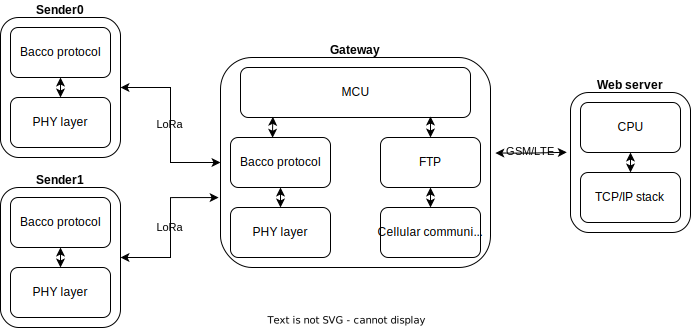
\includegraphics[width=1.0\textwidth]{uml/network_stack.pdf}
    \caption{Schematic representation of an example network using Bacco}
    \label{img: network stack}
\end{figure}

\section{Topology}
The network has a star-of-stars topology, in which the zeroth level is occupied by the Web server, the first level by the
Gateways and Repeaters, and the second level contains the Senders.
Figure \ref{network topology img} shows the type of devices that are involved and their communication schema. \\
The structure is equivalent to a tree, hence we can define a hierarchy for the nodes. The root node is the central web server
and its children nodes are the Gateways. All sender nodes are children of either a Gateway or a Repeater and have no
chlidren, so they correspond to the leaves of the tree.

\begin{figure}[h]
    \centering
    \includegraphics[width=1.0\linewidth]{uml/network_topology.pdf}
    \caption{Example network topology}
    \label{network topology img}
\end{figure}

\section{Addressing}
It is crucial to identify each Sender node in order to contextualize the messages coming to the Gateway node.
This is achieved by assigning them a unique identifier, represented by a natural number in the range $\[1,254\]$.
Address 0 is reserved for the Receiver and address 255 is used as a globally invalid address.
This fact limits the number of Sender nodes connected to a single Gateway to 254 \footnote{This choice is influenced
by the current Italian regulations \colorbox{red}{TODO: Scrivi e inserisci citazione a paragrafo su regolamentazione e
calcolo numero massumo di devices} \cite{CITAZIONE PARAGRAFO REGOLAMENTAZIONE E CALCOLO MASSIMO NUMERO DI DEVICES}
\cite{gazzetta_potenza_868} on duty cycle for the 868MHz band and the fact that most agricultural contexts do not
require a huge amount of sensors}. If necessary, the network can scale up by using additional Gateways.
Note that since Repeaters do not produce messages themselves nor they modify the forwarded ones, they will not be
given an identifier.

\section{Interference mitigation}
The LoRa PHY protocol specification does not fully cover the matter of sharing the communication link between multiple
devices, thus it is necessary to define methods for doing so, in order to minimize interference and achieve
a realiable exchange of information. Different techniques are applied in the domain of both time and frequency.

\subsection{Channel activity detection}
Channel Activity Detection, or CAD, is a feature available with most LoRa transcievers\cite{cad}. In this mode, the LoRa node
listens for any transmission on a specific frequency and, if it detects a signal, an interrupt is returned to the MCU. This
presents a possible Carrier Sense Multiple Access mechanism, also called CSMA.\\
Bacco does not make use of CAD for data packets, but it enables it in specific situations such as network discovery (discussed
in section \ref{Network discovery}).

\subsection{IQ inversion}
IQ inversion is a LoRa primitive that makes it possible to have 2 types of transmissions on the same frequency and
spreading factor, that are easily
distinguishable for a receiver. The name stands for \emph{In-phase / Quadrature}, and it usually refers to
signals that are out of phase from each other by $\frac{\pi}{4}$ rad. Despite that, LoRa uses the term to describe
2 signal with inverted chirp direction, namely up-chirp and down-chirp (see figure \ref{img: iq inversion}).\\
Bacco uses this technique to discriminate between uplink messages (i.e. from Sender to
Gateway/Repeater and fom Repeater to Gateway) and downlink messages (i.e. from Gateway to Sender/Repeater and from
Repeater to Sender). This implies that Sender nodes and Gateway nodes are not able to communicate with other devices of
the same category (e.g. a Sender would not detect any transmission coming from a Sender).

\begin{figure}[h]
    \centering
    \begin{subfigure}[b]{0.45\linewidth}
        \begin{subfigure}[b]{\linewidth}
            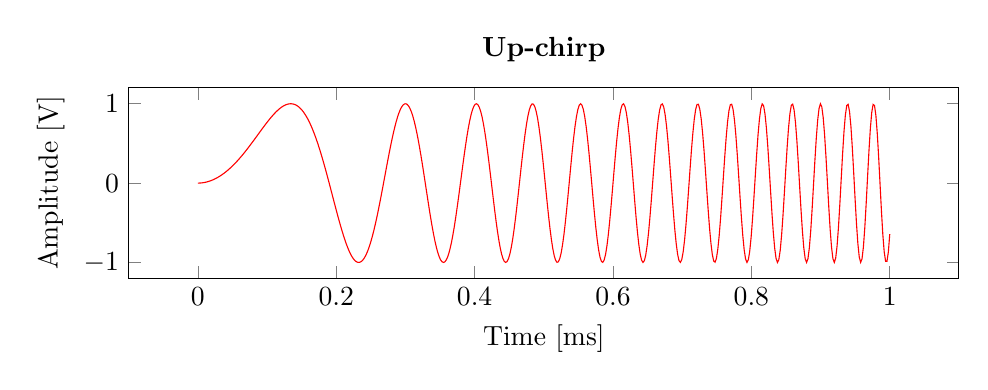
\begin{tikzpicture}
                \begin{axis}[width=\linewidth, height=4cm, title={\textbf{Up-chirp}}, xlabel={Time [ms]}, ylabel={Amplitude [V]}]
                    \addplot[color=red, samples=500][domain=0:1]{sin(x*x*5000)};
                \end{axis}
            \end{tikzpicture}
        \end{subfigure}
        \begin{subfigure}[b]{\linewidth}
            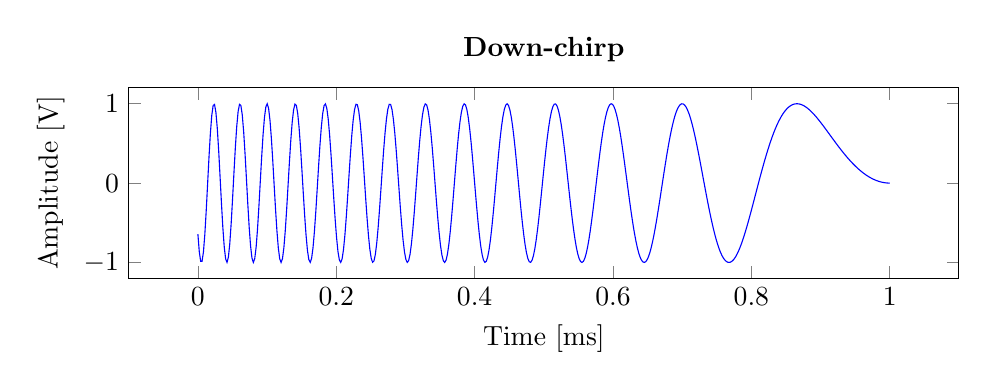
\begin{tikzpicture}
                \begin{axis}[width=\linewidth, height=4cm, title={\textbf{Down-chirp}}, xlabel={Time [ms]}, ylabel={Amplitude [V]}]
                    \addplot[color=blue, samples=500][domain=0:1]{sin(5000*(1-x)*(1-x))};
                \end{axis}
            \end{tikzpicture}
        \end{subfigure}
    \end{subfigure}
    \hspace{0.08\linewidth}
    \begin{subfigure}[b]{0.45\linewidth}
        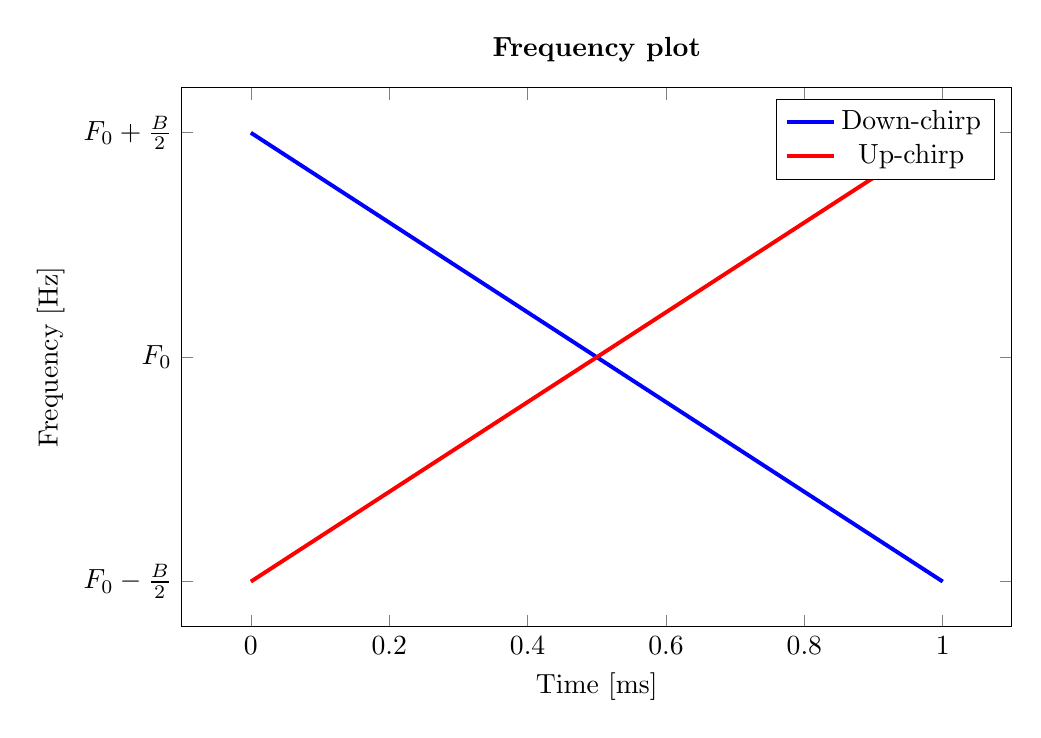
\begin{tikzpicture}
            \begin{axis}[width=\linewidth, height=8cm + \baselineskip, title={\textbf{Frequency plot}}, xlabel={Time
                [ms]}, ylabel={Frequency [Hz]}, ytick={0, 0.5, 1}, yticklabels={$F_0-\frac{B}{2}$, $F_0$, $F_0+\frac{B}
                {2}$}, legend entries={Down-chirp, Up-chirp}]
                \addplot[line width=0.5mm, color=blue, samples=500][domain=0:1]{1-x};
                \addplot[line width=0.5mm, color=red, samples=500][domain=0:1]{x};
            \end{axis}
        \end{tikzpicture}
    \end{subfigure}
    \caption{IQ inversion}
    \label{img: iq inversion}
\end{figure}

\subsection{Subnetting}
The LoRa procol supports a wide range of carrier frequencies in the \gls{VHF} spectrum \footnote{For reference, the
SX1262\cite{sx1262} transciever features a continuous frequency coverage from 150 MHz to 960 MHz}.\\
Bacco exploits this fact to build sub-networks that operate at different frequencies, and thus it achieves a communication with very low
interference between different the independent parts. All the Sender nodes connected to a Repeater and the Repeater
itself operate at a frequency that's different from the frequency used by the Gateway and other Repeaters. Figure \ref{repeaters
subnet} shows a schematic representation. This technique is particularly useful to solve the problem of bouncing, that occours
when a message is sent back to the original Repeater from another Repeater.\\
It is necessary to define a set of frequencies at which the nodes operate. This choice is done
based on current regulations in the specific country of operation; this thesis will focus on Italian and/or European
standards. 868 MHz is the base frequency at which the Gateway node operates. The set of 11 frequencies of operation
is so composed:
\begin{equation}
\label{set of frequencies}
f = \left\{ f_k : f_k = 868\text{MHz} + k \times 125\text{KHz}, k\in \left\{0..10 \right\} \right\}
\end{equation}
This implies that a Bacco network can have up to 10 Repeaters operating at different frequencies, however if more coverage
is needed, it is possible to have multiple Repeater nodes working at the same frequency, given that they are not in
reach with each other.


\begin{figure}[h]
    \centering
    \includegraphics[width=\linewidth]{uml/repeaters_subnet.pdf}
    \caption{Example network with repeaters in subnets}
    \label{repeaters subnet}
\end{figure}


\subsection{Distribution of transmission activity}
The Bacco protocol distributes radio activity over time with defined frames reserved for each Sender, using
an approach that was first introduced by the AlohaNet\cite{alohanet} protocol. The frames are equally distributed between
all the Senders and the start of each of them is function of the identifier. The time delay between 2 consecutive
transmissions from a same Sender is a constant value and it is called cycle. At the end of a cycle, some time is
reserved for the Gateway to upload the collected data. Figure \ref{timing diagram} shows a schematic representation of
the time management used by Bacco. The cycle time is a user-defined parameter, and all the other values are
calculated based on it as shown in table \ref{timing table}. \\

\begin{table}[h]
    \centering
    \setlength{\extrarowheight}{7pt}
    \begin{tabular}{ |c|c| }
        \hline
        \textbf{Parameter} & \textbf{Value}\\
        \hline
        Gateway frame time & $0.2 \cdot C$\\
        Sender frame time & $\frac{0.6 \cdot C}{N_{max}}$\\
        Silence frame time & $\frac{0.2 \cdot C}{N_{max}}$\\
        \hline
    \end{tabular}
    \caption{Time parameters calculation. C is the cycle time and $N_{max} = 254$ is the maximum number of Senders}
    \label{timing table}
\end{table}

\begin{sidewaysfigure}
    \centering
    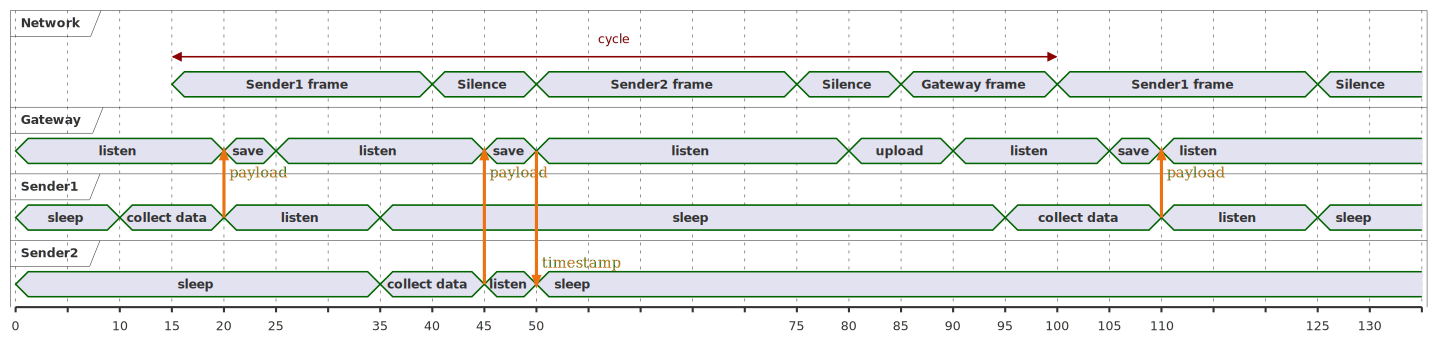
\includegraphics[clip, trim=0cm 25.2cm 0cm 0cm, width=1.0\textwidth]{uml/timings.pdf}
    \caption{Timing diagram}
    \label{timing diagram}
\end{sidewaysfigure}

\subsubsection{Compensating clock drift}
All the devices in the network need to transmit during their assigned frame for the protocol to be effective; this means
that all the clocks of the devices are required to be in sync. This is hard to achieve without dynamic recalibration,
because commercial oscillators cannot provide a constant frequency source due to manifacturing imprecisions,
temperature gradient etc... .\\
In order to deal with with this problem, Bacco assigns the Gateway node the role of coordinating the network timings through
the dispatch of downlink messages containing the network timestamp. A downlink message is sent as soon as the Gateway
receives an uplink message that exceedes its correct time frame. Figure \ref{timing diagram} shows this behavior during
the transmission involving Sender2.
Additionally, the Gateway sends at least 1 downlink message every 10 uplink messages from a same Sender, to
signal that the connection is still active.

\section{Network discovery}
\label{Network discovery}
When a Sender node is first started, it needs to decide at what frequency it has to operate for minimizing the power
needed to reach a Repeater or Gateway. In order to do this, Bacco introduces method \ref{algo:network discovery}
for scanning nearby devices and selecting the most suitable. It tries to establish a communication with Repeaters and
Gateways throughout all the available frequencies by sending a particular type of message that triggers a SYN/ACK
response. CAD will be used by the Sender to not interfere with ongoing communications; this is because the board does
not yet have an allocated time frame and thus cannot decide when to transmit otherwise.

\begin{algorithm}[h]
    \caption{Network discovery}\label{algo:network discovery}
    \begin{algorithmic}

        \State rssi\_values $\gets$ $\[0,0,0,0,0,0,0,0,0,0\]$

        \While{all rssi\_values are equal to 0}
            \For{$k$ from 0 to 10}
                \State $f_k$ $\gets$ $868 \times 10^6 + k \times 125 * 10^3$
                \For{$i$ from 0 to 10}
                    \Do
                        \State sleep for 1 second
                        \State enter CAD mode at frequency $f_k$ for 1.5 seconds
                    \doWhile{activity detected by CAD}
                    \State send sensing message
                    \State enter receive mode for 3 seconds
                    \If{received SYN/ACK}
                        \State $\text{rssi}\_values\[k\]$ $\gets$ current rssi
                        \State \textbf{break}
                    \EndIf
                \EndFor
            \EndFor
        \EndWhile
        \State \textbf{return} $868 \times 10^6 + \text{argmin(rssi\_values)} \times  125 * 10^3$
    \end{algorithmic}
\end{algorithm}


\section{Network joining}
When a Sender node needs to connect to a Gateway node for the first time, it does not yet have an identifier nor is in
sync with the network. The procedure to achieve that will be called the joining process. Note that we assume that the
Sender node has already selected its frequency of operation, as descibed in section \ref{Network discovery}.\\
We will ignore the act of forwarding made by any optional Repeater node, as in this case it does not affect the
content of the messages, but note that delay and error rate would raise in that situation. All the messages sent from Sender
and Receiver make use of CAD to make sure the channel is free before the actual transmission; this step will be omitted
in the description for brevity. First, the Sender transmits a SYN message to the Gateway and waits for a SYN/ACK
response for 3 seconds. If no message is received, another SYN message is sent for a maximum of 10 times. After that,
the Gateway waits for 3 seconds for an ACK message from the Receiver, and if no message is received it will try again
for a maximum of 10 times. The SYN/ACK message contains the timestamp of the network as well as the assigned identifier.
If the maximum number of iterations is reached in any of the steps, the process starts again after 30 minutes.
Figure \ref{img: network joining} show a schematic representation of the process.

\begin{figure}[h]
    \centering
    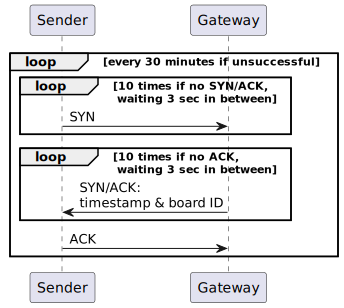
\includegraphics[width=200pt]{uml/network_joining.pdf}
    \caption{Network joining process}
    \label{img: network joining}
\end{figure}

\section{Downlink commands}
In some situations (e.g. \ref{sec: transmission power adaption}), it is required to be able to change the behavior of the
network dynamically and in a reliable way. Bacco achieves this by exhanging specialized kind of packets that contain a
command. Each command message needs to be acknowledged by the Sender to the Gateway/Repeater in a similar way as done during the
network joining procedure. Figure \ref{img: command ack} offers a graphical representation of the process.\\
The following commands are defined by the protocol, and each of them is associated to an opcode as shown in table
\ref{tab: opcodes}:
\begin{description}[font=$\bullet$~\normalfont\scshape\color{blue!50!black}]
    \item [Shutdown] - If this command is sent and processed successfully, the Sender goes to sleep indefinetly until a
        manual reset is invoked by pressing a physical button
    \item [Enter quiescent mode] - If this command is processed successfully, the Sender stops to send data, but it keeps
        listening for incoming messages/commands during its time frame
    \item [Wakeup] - If this command is processed successfully, the Sender enters normal/active mode
        and thus starts to transmit data
    \item [Increase transmission power] - If this command is processed successfully, the Sender increases its
        transmit power by 3dBm
    \item [Decrease transmission power] - If this command is processed successfully, the Sender deceases its
        transmit power by 3dBm
\end{description}

\begin{table}[h]
    \centering
    %\setlength{\extrarowheight}{5pt}
    \begin{tabular}{ |c|c| }
        \hline
        \textbf{Command} & \textbf{Opcode as 7 bit unsigned integer}\\
        \hline
        Shutdown & 0\\
        \hline
        Enter quiscent mode & 1\\
        \hline
        Wakeup & 2\\
        \hline
        Increase transmission power & 3\\
        \hline
        Decrease transmission power & 4\\
        \hline
        Reserved for later use & [4-50]\\
        \hline
        User defined & [51-127]\\
        \hline
    \end{tabular}
    \caption{Table of opcodes}
    \label{tab: opcodes}
\end{table}

\begin{figure}[h]
    \centering
    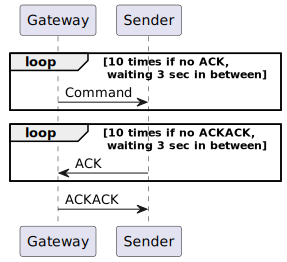
\includegraphics[width=200pt]{uml/command_ack.pdf}
    \caption{Command sending process}
    \label{img: command ack}
\end{figure}

\section{Transmission power adaption}
\label{sec: transmission power adaption}
Since Senders can be placed at different distances from a Gateway or Repeater, it is useful to optimize the power
used by the node to transmit. The default value for the transmission power is equal to $P_{0}$; starting from that, the
network will automatically drift towards a more suitable value according to the
following triggers:
\begin{itemize}
    \item If a Sender has not received any downlink messages during
        the last 20 frames, then its transmission power will be increased by $P_{step}$
    \item If 9 out of the last 10 messages received by a Repeater or a Gateway
        satisfy $\text{RSSI} > \text{RSSI}_{high}$ and $\text{SNR} > \text{SNR}_{high}$, then
        a command is sent to the Sender telling to decrease its transmission power by $P_{step}$
    \item If 9 out of the last 10 messages received by a Repeater or a Gateway
        satisfy $\text{RSSI} < \text{RSSI}_{low}$ or have not been received, then a command is sent to the Sender telling to
        increase its TX power by $P_{step}$.
\end{itemize}
The values for the used parameters are shown here:
\begin{equation}
    \begin{array}{l}
        P_{0} = P_{max} = 14\text{ dBm} \\ P_{step} = 3\text{ dBm} \\ \text{RSSI}_{low} = -115\text{ dBm} \\ \text{RSSI}
        _{high} = -60\text{ dBm} \\ \text{SNR}_{low} = -7\text{ dBm}
    \end{array}
\end{equation}
Gateways and Repeaters always operate at $P_{0}$, since power efficiency is less critical than reliability for such nodes.


\section{Packet format}
In this section the bit format of the messages is shown. The analysis will be split betqween uplink packets and downlink
packets.

\subsubsection{Uplink packet format}
An uplink message is sent from a Sender to a Gateway/Repeater or from a Repeater to a Gateway. It has a variable
length and it is transmitted using up-chirps, i.e with IQ inversion disabled. Figure \ref{img: uplink packet format} shows its
format.

\begin{figure}[h]
    \centering
    \begin{bytefield}[]{32}
        \bitheader{0,8,16} \\
        \bitbox{8}{Sender ID} & \bitbox{8}{Payload size}
                              & \bitbox{16}{Payload}
    \end{bytefield}
    \caption{Uplink packet format}
    \label{img: uplink packet format}
\end{figure}


\subsubsection{Downlink packet format}
A downlink message is sent from a Gateway to a Sender/Repeater or from a Repeater to a Sender. It has a fixed
length of 5 bytes and it is transmitted using down-chirps, i.e with IQ inversion enabled. Figure \ref{img: downlink
packet format}, \ref{img: downlink timestamp packet format}, \ref{img: downlink command packet format} show the
general format, the timestamp format and the command format respectively.

\vspace{1.6cm}
\newcommand{\bitlabel}[2]{%
    \bitbox[]{#1}{%
        \raisebox{0pt}[4ex][0pt]{%
            \turnbox{65}{\fontsize{9}{9}\selectfont#2}%
        }%
    }%
}
\begin{figure}[h]
    \centering
    \begin{bytefield}[]{40}
        \bitlabel{8}{} & \bitlabel{1}{Message type} & \bitlabel{31}{}\\
        \bitheader{0,8,9,39} \\
        \bitbox{8}{Sender ID} & \bitbox{1}{}
                              & \bitbox{31}{Payload}
    \end{bytefield}
    \caption{Downlink packet format}
    \label{img: downlink packet format}
\end{figure}

\begin{figure}[h]
    \centering
    \begin{bytefield}[]{40}
        \bitheader{0,8,9,39} \\
        \bitbox{8}{Sender ID} & \bitbox{1}{0}
                              & \bitbox{31}{Timestamp}
    \end{bytefield}
    \caption{Downlink packet format of timestamps}
    \label{img: downlink timestamp packet format}
\end{figure}

\begin{figure}[h]
    \centering
    \begin{bytefield}[]{40}
        \bitheader{0,8,9,16,39} \\
        \bitbox{8}{Sender ID} & \bitbox{1}{1}
                              & \bitbox{7}{Opcode}
                              & \bitbox{24}{Padding}
    \end{bytefield}
    \caption{Downlink packet format for commands}
    \label{img: downlink command packet format}
\end{figure}



\chapter{Performance}
\label{chapter:performance}
The goal of this chapter is to discuss the performance of Bacco, using a variery of parameters, methods and laboratory
tests. The results will also be compared to the ones obtained by applying the same procedures to devices using the
LoRaWAN protocol.

\section{Time On Air And Duty Cyle}
\Gls{ToA} is a crucial metric to take into consideration when measuring the performance of a network protocol. It is
defined as time that a device takes to transmit a packet on the channel. At the same conditions, a shorter \gls{ToA}
results in improved energy efficiency and smaller probability of interference with packets transmitted from other
devices.\\
\Gls{ToA} is correlated to the packet lenght in symbols (a longer packet will require a longer trasmission time).
Referencing the official LoRa documentation, see \cite{sx1262}, we can find that \gls{ToA} is
discussed in section 6.1.4; in particular the exact formula is shown here by Equation \ref{eqn: ToA}.
\begin{equation}
    \label{eqn: ToA}
    \mathit{ToA} = \frac{2^{\mathit{SF}}}{\mathit{BW}}*\mathit{N_{symbols}}
\end{equation}

where
\begin{itemize}[noitemsep,nolistsep]
    \item[\boldmath$\cdot$] $\mathit{SF}$ is the Spreading Factor (from 5 to 12);
    \item[\boldmath$\cdot$] $\mathit{BW}$ is the Bandwidth (in kHz);
    \item[\boldmath$\cdot$] $\mathit{N_{symbols}}$ is the number of symbols in the packet.
\end{itemize}
\\
$\mathit{N_{symbols}}$ can be calculated knowing the bytes of the packet ($\mathit{N_{bytes_{payload}}}$) using Equation \ref{eqn: n_symbols SF5_6} for $\mathit{SF} \in \left
\{5, 6 \right\} $ and Equation \ref{eqn: n_symbols SF7_12} for $\mathit{SF} \in \left
\[7, 12 \right\] $

\begin{equation}
    \label{eqn: n_symbols SF5_6}
    \resizebox{.9\hsize}{!}{
    \mathit{N_{symbols}} = \mathit{N_{symbols_{preamble}}} + 6.25 + 8 + \textit{ceil} \left( \frac{\textit{max} \left( 8 *
        \mathit{N_{bytes_{payload}}} + \mathit{N_{bits_{CRC}}} - 4 * \mathit{SF} + \mathit{N_{symbols_{header}}},
0 \right) }{\mathit{SF} * \mathit{CR}} \right)}
\end{equation}

\begin{equation}
    \label{eqn: n_symbols SF7_12}
    \resizebox{.9\hsize}{!}{
    \mathit{N_{symbols}} = \mathit{N_{symbols_{preamble}}} + 4.25 + 8 + \textit{ceil} \left( \frac{\textit{max} \left( 8 *
        \mathit{N_{bytes_{payload}}} + \mathit{N_{bits_{CRC}}} - 4 * \mathit{SF} + 8 + \mathit{N_{symbols_{header}}},
0 \right) }{\mathit{SF} * \mathit{CR}} \right)}
\end{equation}

where
\begin{itemize}[noitemsep,nolistsep]
    \item[\boldmath$\cdot$] $\mathit{N_{bits_{CRC}}}$ is number of bits used for \gls{CRC} and can assume a value of
        either 0 or 16;
    \item[\boldmath$\cdot$] $\mathit{N_{symbols_{header}}}$ is the number of symbols in the packet header.
        Since each symbol encodes $\mathit{SF}$ bits, $\mathit{N_{symbols_{header}}} = \frac{\mathit{N_{bits_{header}}}}
        {\mathit{SF}}$;
    \item[\boldmath$\cdot$] $\mathit{CR}$ is the coding rate and can assume a value of either $\frac{4}{5},\frac{4}{6},
        \frac{4}{7}$ or $\frac{4}{8}$.
\end{itemize}
\vspace{0.55cm}
The duty cycle is the fraction of time in which the channel is busy, it can be calculated using Equation \ref{eqn: duty cycle}.
\begin{equation}
    \label{eqn: duty cycle}
    d = \frac{\tau}{T}
\end{equation}
where
\begin{itemize}[noitemsep,nolistsep]
    \item[\boldmath$\cdot$] $d$ is the duty cycle;
    \item[\boldmath$\cdot$] $\tau$ is the \gls{ToA};
    \item[\boldmath$\cdot$] $T$ is the transmission period.
\end{itemize}
\\

\subsection{Regulations}
\label{subsec: regulations}
In order to maintain a fair distribution of the transmission activity, local, national and international governments
define limits on the usage of the radio channel. The limits vary by the frequency band in which the devices operate at.
The two parameters that are often used as an upper bound not to be crossed are \gls{ERP}\footnote{\gls{ERP} is the
measure of the power effectively radiated by an antenna system in a specific direction, accounting for both transmitter
output and antenna characteristic. It is commonly expressed in watts or decibel and it is used for determining the coverage area
and range of a radio.} and duty cycle.\\
Using the current Italian regulations at the time of writing as an example, we can observe that the spectrum is split into
frequency bands that can be either free, reserved or restricted; each of them has three parameters associated to it: the
maximum \gls{ERP}, the minimum channel bandwidth and the maximum duty cycle. The official document
that discusses this matter in detail can be found in \cite{gazzetta_potenza_868}. The bands that LoRa devices use in
Europe are $\[868.0,868.6\]$ MHz and $\[868.7,869.2\]$ MHz, they both feature a maximum \gls{ERP} of 25 mW or 14 dBm and
do not have any restriction on channel bandwidth, however the first band has a maximum duty cycle of 1\%, while for the
other the limit is set to 0.1\%.\\ An important fact to point out is that the limits apply to a physical person or
organization and not to on a device basis, so to calculate the effective duty cycle, we have to consider the
transmission activity generated by the whole network.

\subsection{Maximum Number Of Devices In A Network}
We can now calculate the maximum number of devices that can be operational at the same time. To achieve that, we can
derive Equation \ref{eqn: max devices rev} from Equation \ref{eqn: ToA} and then maximize the number of devices
($\mathit{N_{devices_{max}}}$), getting Equation \ref{eqn: max devices}.
\begin{equation}
    \label{eqn: max devices rev}
    \frac{\tau * \mathit{N_{devices}}}{T} \leq \mathit{d_{max}}
\end{equation}
\begin{equation}
    \label{eqn: max devices}
    N_{devices_{max}} = \textit{floor} \left( \frac{\mathit{d_{max}} * T}{\tau} \right)
\end{equation}
where
\begin{itemize}[noitemsep,nolistsep]
    \item[\boldmath$\cdot$] $T$ is the transmission period and can be set arbitrarily;
    \item[\boldmath$\cdot$] $\tau$ can be computed using Equation \ref{eqn: ToA};
    \item[\boldmath$\cdot$] $\mathit{d_{max}}$ is the maximum duty cycle, it has to be smaller or equal to 1 and can be
        set accordingly to the local regulations or the specific needs.
\end{itemize}
\\

\subsubsection{Example Of Calculation}
To demonstrate the use of the Equation \ref{eqn: max devices}, we will now consider a network with the following
properties:
\begin{itemize}
    \item each Sender node has a transmission period of $T = 1 \textit{ hour} = 3600\ s$;
    \item each Sender node transmits a packet with a payload that has a lenght in bytes equal to $\mathit{N_{bytes_{payload}}} = 16$;
    \item the network operates at a frequency of 868.0 Mhz on the Italian territory, and thus has to respect the limit
        of $\mathit{d_{max}} = 1\% = 0.01$.
\end{itemize}


\subsubsection{Bacco}
a downlink is sent every 10 packets;

\subsubsection{LoRaWAN}
a downlink is sent every packet (confirmation);


\section{Laboratory Tests}

\subsection{Single Packet Energy}

\begin{figure}[ht]
    \centering
    \includegraphics[width=1.0\textwidth]{images/bacco_SF7_14dbm_125khz_power.pdf}\\
    \vspace{-0.7cm}
    \includegraphics[width=1.0\textwidth]{images/lorawan_SF7_14dbm_125khz_power.pdf}
    \caption{Power draw of Bacco (in red) and LoRaWAN (in blue) during the transmission of a packet with a payload of 15
    bytes, using SF7, 14dBm, 125kHz bandwidth}
    \label{bacco SF7}
\end{figure}

Bacco:\\
delta time is 51.6ms and total energy is 21.3mJ
\\\\
LoRaWAN:\\
delta time is 71.8ms and total energy is 30.8mJ

\subsection{Packet Error Rate}
Crunch some fking data from FTP server

4 lost packets for every 1008 packets (0.4\% biatcz)
%TODO: similar test with fking LoRa fking WAN


%\chapter{Conclusions}
%\label{chapter:conclusions}
%\input{conclusions.tex}

% Bibliography
%\clearpage{\pagestyle{plain}\cleardoublepage}
%\begin{thebibliography}{99}
\addcontentsline{toc}{chapter}{Bibliography}

\bibitem{Principles of GSM} "Principles and Applications of GSM" by \\ \url{https://dl.acm.org/doi/abs/10.5555/552293}

\bibitem{FTP rfc} FTP request for comments specification\\ \url{https://www.rfc-editor.org/rfc/rfc959.html}

%\bibitem{sklearnArt}Buitinck L., Louppe G., Blondel M., Pedregosa F., Mueller A., Grisel O., Niculae V., Prettenhofer P., Gramfort A., Grobler J., Layton R., Vanderplas J., Joly A., Holt B., Varoquaux G., \textit{API design for machine learning software: Experiences from the scikit-learn project}, 2013.

%\bibitem{CNN} \textit{Convolutional Neural Networks}, \url{http://deeplearning.net/tutorial/ lenet.html}, last consultation: 07/01/2020.

\end{thebibliography}

\addbibresource{refs.bib}

\nocite{*}
\printbibliography
\end{document}

%Examples

%\clearpage{\pagestyle{plain}\cleardoublepage} %Start chapter on an odd numbered page
%\chapter{Bytefields} %Chapter name
%\label{chapter:bytefields} %Label for references
%\input{bitfields.tex} %File for the actual chapter


%\clearpage{\pagestyle{plain}\cleardoublepage}
%\chapter{First Chapter}
%\label{chapter:primo_capitolo}
%\input{intro_cap1.tex}

%\clearpage{\pagestyle{plain}\cleardoublepage}
%\chapter{Tables and images}
%\label{chapter:immagini_e_tabelle}
%Metodi più comuni per inserire immagini e esempi di tabelle.

\section{Immagine singola}
\input{imgs_tables/immagine_singola.tex}

\section{Immagine multipla}
\input{imgs_tables/immagine_mul.tex}

\section{Tabelle}
\input{imgs_tables/tabelle.tex}


%\clearpage{\pagestyle{plain}\cleardoublepage}
%\chapter{Formulas}
%\label{chapter:formule}
%\input{intro_cap3.tex}

%\clearpage{\pagestyle{plain}\cleardoublepage}
%\chapter{Pseudocode and code}
%\label{chapter:codice}
%\input{intro_cap4.tex}

